\documentclass[../main.tex]{subfiles}

\begin{document}
\section{Results}\label{sec: results}
In this section we go over our results of the European Call Option and compared our result from classical to the quantum result.
For that we used the following parameters $S_0 = 2, \sigma = 0.4, r=0.05, T=40/365, K=2, n=3, c=0.25$, $n$ is the number of qubits.
The log-normal distribution is then constructed by using $\mu = (r-0.5 \cdot \sigma^2) \cdot T + log(S_0)$ and $\sigma_{\text{dist}} = \sigma \cdot \sqrt{T}$.
For the stockprices we chosed the values to lay between the low boundary $l = \max (0, \mu - 3 \cdot \text{stddev})$ and the high value $h = \mu + 3\cdot \text{stddev} $.
In fig. (\ref{fig:E_log-normal}) the resulting log-normal distribution can be seen.
\begin{figure}[H]
  \begin{center}
    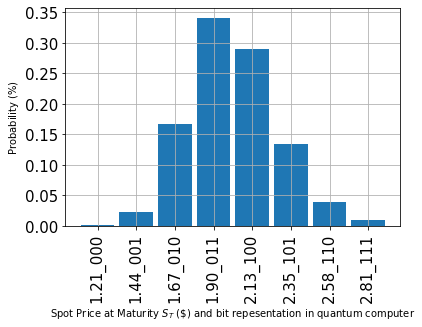
\includegraphics[width=0.5\linewidth]{../../images/probability.png}
  \end{center}
  \caption{The distinct log-normal distribution (eq. \ref{eq:lognormal}), with $\mu=(r-0.5\cdot \sigma^2)\cdot T + \log(S_0)$, $\sigma_{\text{dist}}=\sigma \cdot \sqrt{T}$ and as lower $l$ and highest $h$ value we used the 3 standard deviation. As x value the classical value is shown and the corresponding qubit state which are representing the number in our quantum computer.}
  \label{fig:E_log-normal}
\end{figure}

Remember that the equation for the european payoff function is
\begin{align}
    F(S(T)) = \max\{0, S(T) - K\} \label{eq:E_example_european}
\end{align}
and creates the piecewise linear function shown in figure \ref{fig:E_payoff_function}.
\begin{figure}[H]
  \begin{center}
    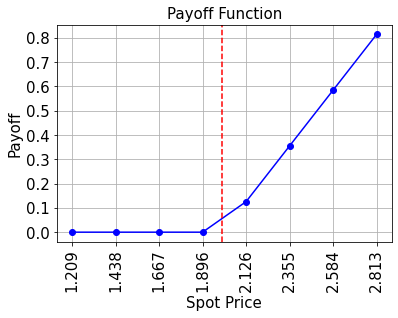
\includegraphics[width=0.5\linewidth]{../../images/payoff_european.png}
  \end{center}
  \caption{Visaulization of the piecewise-linear payoff functions. Breakpoints are set to $[0, 2.126]$ or $[\ket{000}, \ket{100}]$ 
  thanks to ceil operation described in \ref{sec:ImplPieceFunc}}
  \label{fig:E_payoff_function}
\end{figure}
Together with the discussion around \ref{sec:ImplMaxFunc} the application of payoff function to the given circuit is displayed in
Fig. \ref{fig:E_model_payoff_function}. 
\begin{figure}[H]
  \begin{center}
    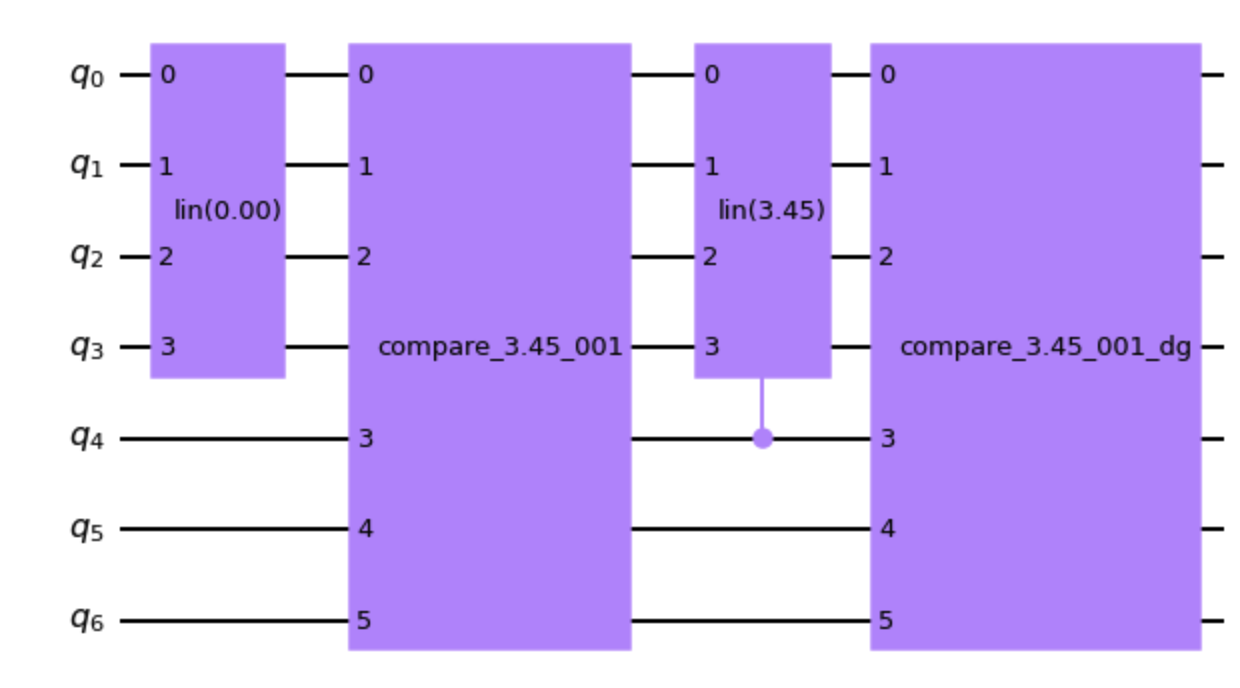
\includegraphics[width=\linewidth]{../../images/Agate.png}
  \end{center}
  \caption{The payoff gate or equivalent to operater $A$ in Fig. \ref{fig:qae}. 
  The circuit is divided in four sections. 
  The first section is the $Y$-Rotation for the first breakpoint.
  The second section is the comparator for the second breakpoint. 
  The next section is then the controlled rotation for values above the second breakpoint.
  It is good to see that the fourth qubit is used to decide if the rotation should be executed or not.
  The last section is the inverse of the second section.}
  \label{fig:E_model_payoff_function}
\end{figure}
Measuring all qubits in computational basis the result shown in Fig. \ref{fig:E_probability_estimate}.
 \begin{figure}[H]
  \begin{center}
    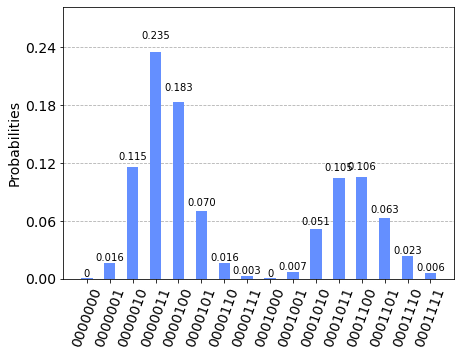
\includegraphics[width=0.5\linewidth]{../../images/probability_estimate.png}
  \end{center}
  \caption{Measurement outcome after applying the payoff function to the circuit. above}
  \label{fig:E_probability_estimate}
\end{figure}

The Grover operator $\mathcal{Q}=AS_0A^\dagger S_{\psi_1}$ can now be constructed and used for phase estimation part of amplitude estimation. 

For european call options the $A$-gate of the Grover operator is the circuit shown in figure \ref{fig:E_model_payoff_function}, $A^{\dagger}$ is simply the complex conjugate of $A$. 
$S_0$ is realized by a bit-flip of the objective qubit $q_3$ sandwiched by H-gates. $S_{\psi_1} = 1-2\ket{\psi_1}\ket{0}\bra{\psi_1}\bra{0}$ is implemented using $2\ket{\psi_1}\ket{0}\bra{\psi_1}\bra{0}-1$
and a global phase bit, since the negative form can easily be implemented by using multi-controlled Z-gates sandwiched by X-gates on the target qubit. 
The global phase has no effect on Grovers algorithm in general. The Grover is shown in figure \ref{fig:grover}

 \begin{figure}[H]
  \begin{center}
    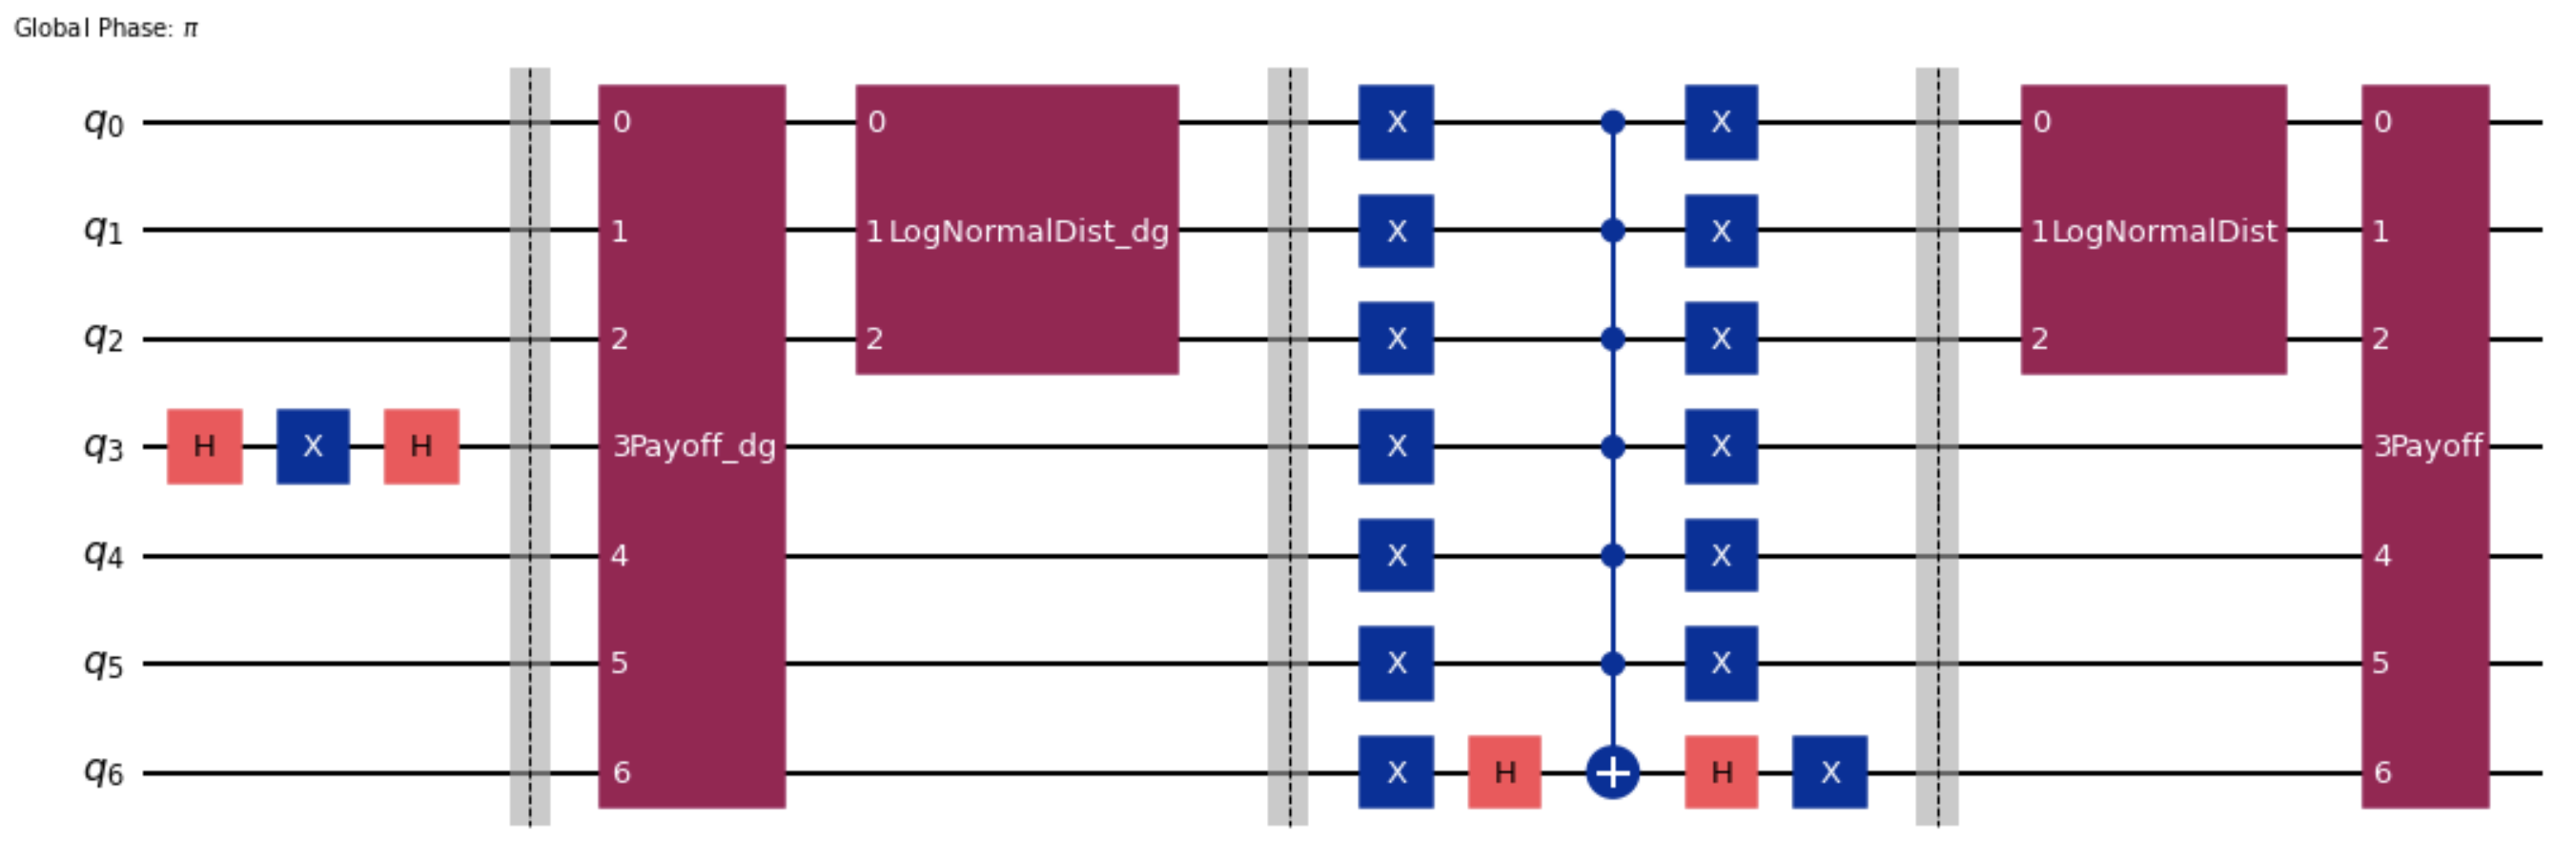
\includegraphics[width=\linewidth]{../../images/grover.png}
  \end{center}
  \caption{The Grover-operator. $S_0$ is a bit-flip implemented by a X-gate sandwiched by H-gates. $A$, $A^{\dagger}$ is the circuit and its complex-conjugate shown in figure $\ref{fig:E_model_payoff_function}$.\\
  $S_{\psi_1} = 1-2\ket{\psi_1}\ket{0}\bra{\psi_1}\bra{0}$ is implemented using $2\ket{\psi_1}\ket{0}\bra{\psi_1}\bra{0}-1$ and a global phase bit.}
  \label{fig:grover}
\end{figure}
 \begin{figure}[H]
  \begin{center}
    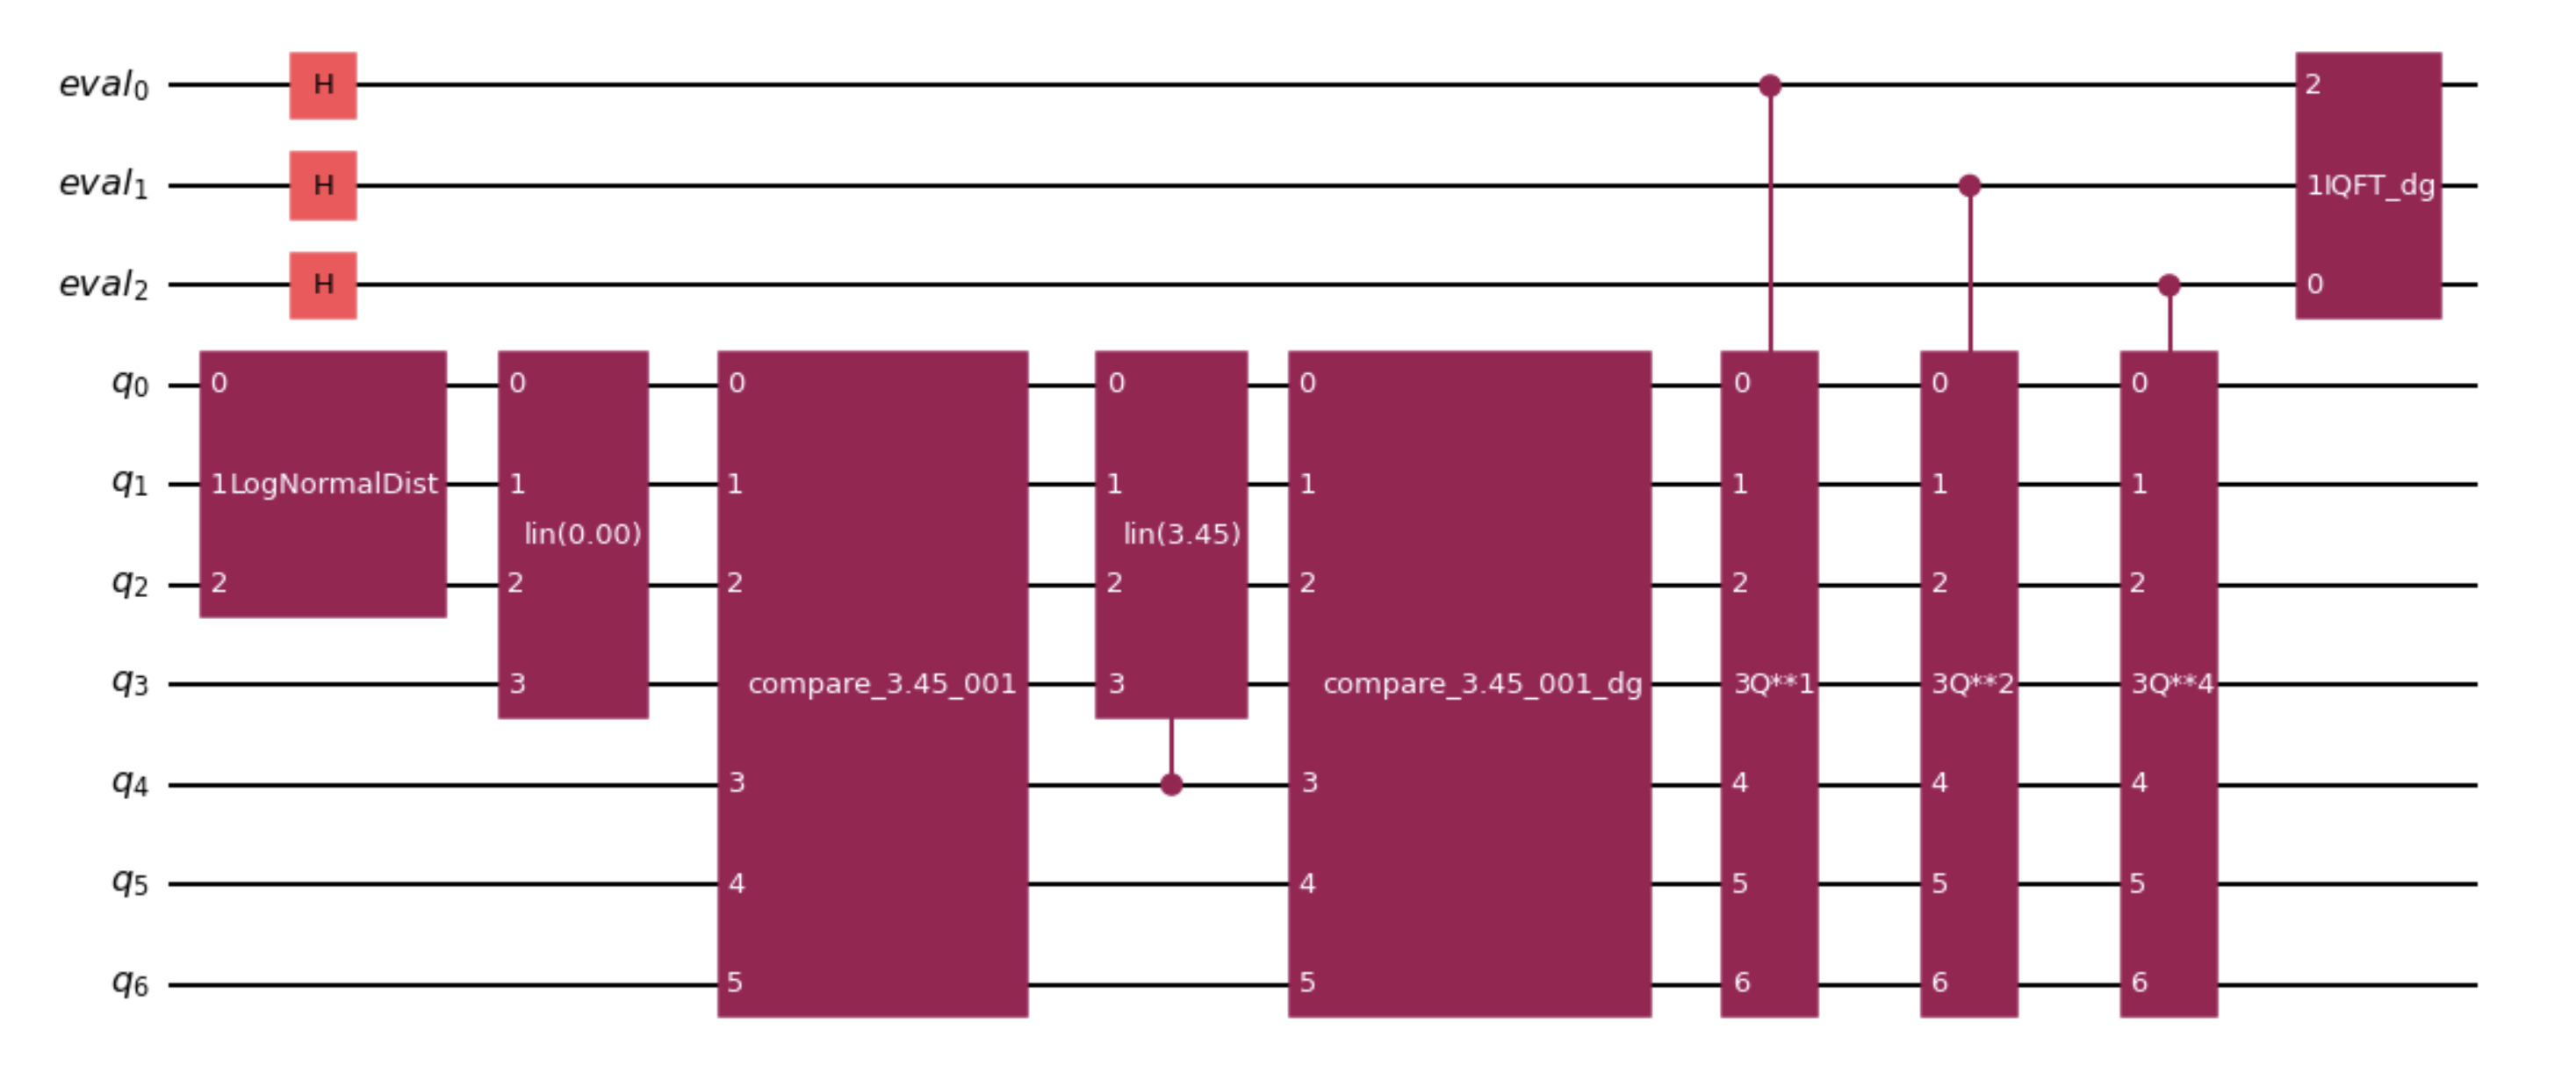
\includegraphics[width=\linewidth]{../../images/combinedCircuit.png}
  \end{center}
  \caption{The combined circuit. Note that the objective qubit here is qubit 3. 
  Three evaluation qubits are chosen for pragmatical reasons. For results a register consisting of seven qubits have been used.}
  \label{fig:combinedCircuit}
\end{figure}
Using the grover operator the combined circuit is displayed in figure $\ref{fig:combinedCircuit}$. 
For the obtained results, i.e. the estimate $\tilde{a}$ seven qubits in the evaluation register have been used. 
Measuring all qubits in the evaluation register gives the following result:
\begin{align}
    &\text{Exact Value: } &0.1133\\
    &\text{Estimated Value: } &0.1061\\
    &\text{95 Percent Confidence interval:	} &[0.1157, 0.1209]
\end{align}
Therefore the estimated value is close to the exact value.//
When we now execute the same circuit for the payoff using iterative amplitude estimation \cite{Grinko_2021}  (i.e. without phase estimation) from qiskit we get the following results:
\begin{align}
    &\text{Exact Value: } &0.1133\\
    &\text{Estimated Value: } &0.1676\\
    &\text{95 Percent Confidence interval:	} &[0.1615, 0.1737]
\end{align}
Which is comparable to the values from canonical amplitude estimation but comes with a lower cost, since iterative amplitude estimation estimates the amplitude without the usage of phase estimation and therefore with less qubits and gates.
\biblio
\end{document}